\section{约束几何与 Lagrange 乘子}
\label{sec:02-Calculus/06-Multivariable-Calculus/06}

给模型加权重衰减时，我们写的是
\[
\min_{\mathbf w}\;L(\mathbf w)+\lambda\norm{\mathbf w}^2 .
\]
可最初想说的往往是另一句话：在``权重别太大''的限制下把损失压到最低，也就是
\[
\min_{\mathbf w}\;L(\mathbf w)
\qquad\text{subject to}\qquad
\norm{\mathbf w}^2\le C .
\]
这两个式子长得不像，实践中却当同一件事用，而且没人真的去调那个 \(C\)，大家调的是 \(\lambda\)。它们凭什么等价？\(\lambda\) 到底是什么量，为什么它有资格代替一个预算？

答案是一个纯几何的观察，本节的其余部分都是它的展开。

\subsection{能走的方向少了，最优的条件也跟着松}

先把场景简化。目标是 \(f(x,y)\)，脚下只有一条既定的路 \(g(x,y)=c\)，不许偏离。无约束时最优要求 \(\nabla f=\mathbf 0\)，即所有方向的一阶变化都归零。现在你根本走不了大部分方向——法向那一侧是禁区，\(f\) 在那里怎么变与你无关。

所以要求应当削弱成：\(f\) 沿约束曲线的\emph{切向}不再变化。用方向导数的语言，对每个切向量 \(\mathbf v\) 都有 \(\ip{\nabla f}{\mathbf v}=0\)。而 \(\nabla f\) 与所有切向量正交，只能意味着 \(\nabla f\) 自己也躺在法向上。

法向是什么？讲梯度时已经证过，\(\nabla g\) 垂直于 \(g\) 的水平集。在平面上法向只有一维，两个都在法向上的向量必成倍数关系：
\[
\nabla f=\lambda\,\nabla g .
\]

这就是 Lagrange 条件的全部来源，它不过是``切向不可改进''换了个写法。几何上它说的是：在最优点处，目标的等高线与约束曲线\emph{相切}。相交而不相切，就说明沿约束还能滑向更好的等高线。

\begin{center}
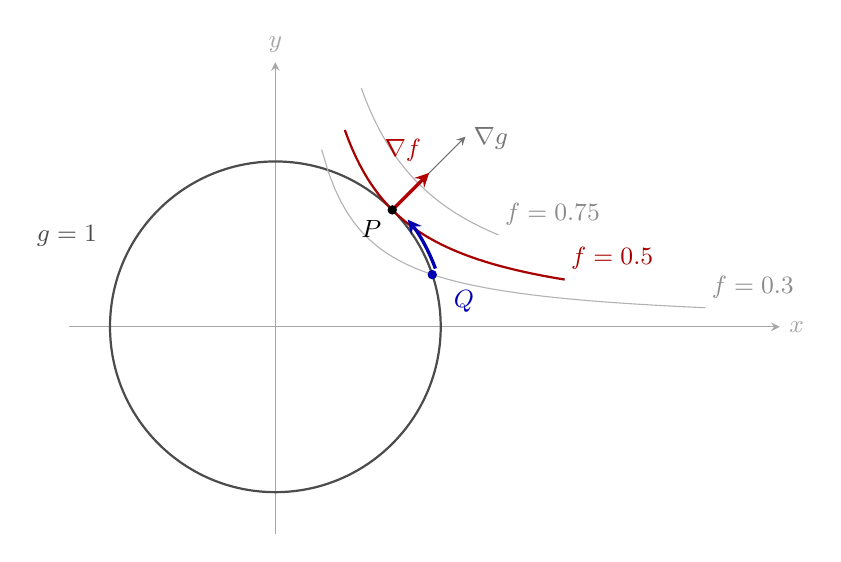
\begin{tikzpicture}[x=2.1cm,y=2.1cm,font=\small,>=stealth]
  \draw[->,black!35] (-1.25,0) -- (3.05,0) node[right] {\(x\)};
  \draw[->,black!35] (0,-1.25) -- (0,1.60) node[above] {\(y\)};
  \draw[black!70,thick] (0,0) circle (1);
  \draw[black!30] plot[domain=0.28:2.60,samples=60] (\x,{0.3/\x});
  \draw[red!65!black,thick] plot[domain=0.42:1.75,samples=60] (\x,{0.5/\x});
  \draw[black!30] plot[domain=0.52:1.35,samples=60] (\x,{0.75/\x});
  \node[above right,black!45] at (2.58,0.115) {\(f=0.3\)};
  \node[above right,red!65!black] at (1.73,0.286) {\(f=0.5\)};
  \node[above right,black!45] at (1.33,0.556) {\(f=0.75\)};
  \node[left,black!70] at (-1.02,0.55) {\(g=1\)};
  \draw[->,black!55] (0.707,0.707) -- (1.15,1.15);
  \draw[->,red!70!black,very thick] (0.707,0.707) -- (0.93,0.93);
  \fill (0.707,0.707) circle (1.7pt);
  \node[below left] at (0.70,0.70) {\(P\)};
  \node[right,black!55] at (1.14,1.14) {\(\nabla g\)};
  \node[above left,red!70!black] at (0.94,0.94) {\(\nabla f\)};
  \fill[blue!70!black] (18.4:1) circle (1.7pt);
  \node[below right,blue!70!black] at (1.02,0.28) {\(Q\)};
  \draw[->,blue!70!black,very thick] (20:1.03) arc (20:39:1.03);
\end{tikzpicture}

\emph{在 \(Q\)（蓝点）处等高线穿过约束圆，目标梯度在切向留有分量，顺着圆走就能爬到更高的等高线。到了相切点，切向分量恰好归零，两个梯度共线——这就是 \(\nabla f=\lambda\nabla g\)。而 \(f=0.75\) 那条等高线整个够不着约束圆，说明 \(0.5\) 已经是这条圆上的上限。}
\end{center}

\begin{example}
在单位圆 \(x^2+y^2=1\) 上求 \(f=xy\) 的最值。\(\nabla f=(y,x)\)、\(\nabla g=(2x,2y)\)，方程组为 \(y=2\lambda x\)、\(x=2\lambda y\) 以及约束本身。第一式乘 \(x\)、第二式乘 \(y\)，右端都是 \(2\lambda xy\)，于是 \(x^2=y^2\)，代回约束得四个候选点 \((\pm1/\sqrt2,\pm1/\sqrt2)\)。同号两点给 \(1/2\)，异号两点给 \(-1/2\)。单位圆紧致而 \(f\) 连续，最值必定取到，所以最大 \(1/2\)、最小 \(-1/2\)。
\end{example}

这个例子顺手暴露了方法的边界：Lagrange 方程只负责生产候选，从不承诺候选是极值，也不承诺候选已经穷尽。判定最值那一步靠的是紧致性加连续性，与乘子无关。

\subsection{\texorpdfstring{\(\lambda\) 是把约束松一格的价格}{lambda 是把约束松一格的价格}}

现在回到开头的问题。把约束水平从 \(c\) 挪到 \(c+\varepsilon\)，最优值也会跟着挪。在适当的正则条件下（最优解光滑地依赖于 \(c\)，且 \(\nabla g\ne\mathbf0\)），这个变化率恰好是乘子：
\[
\frac{d}{dc}\,f\bigl(\mathbf x^\star(c)\bigr)=\lambda .
\]

推一遍就明白它为什么成立。记 \(p(c)=f(\mathbf x^\star(c))\)，链式法则给出 \(p'(c)=\ip{\nabla f}{\tfrac{d\mathbf x^\star}{dc}}\)；把 \(\nabla f=\lambda\nabla g\) 代进去得 \(\lambda\ip{\nabla g}{\tfrac{d\mathbf x^\star}{dc}}\)；而对恒等式 \(g(\mathbf x^\star(c))=c\) 两边求导，那个内积等于 \(1\)。所以 \(p'(c)=\lambda\)。整个论证只用了一次链式法则和一次约束求导。

经济学把它叫影子价格：约束放松一单位，目标能改善多少。它是局部的边际量，不能拿一个点上的 \(\lambda\) 外推到远处；符号也取决于约束写成 \(g=c\) 还是 \(-g=-c\)，读别人的推导时先看约定。

买菜的时候我们其实都在用这个原理。预算就这么多，要在肉和菜之间分配；分得好不好，看最后一元钱就知道——如果它花在肉上比花在菜上更值，那就该从菜那边挪一元过来，直到花在两边一样值为止。这个``一元钱的价值''就是 \(\lambda\)：预算多给一元，这顿饭就好上大约 \(\lambda\) 那么多。

权重衰减的谜团到这里散了。在 \(\min L\) s.t. \(\norm{\mathbf w}^2\le C\) 的最优点上（假定约束是紧的），一阶条件给出 \(\nabla L+\lambda\nabla\norm{\mathbf w}^2=\mathbf 0\)，这正是无约束问题 \(L(\mathbf w)+\lambda\norm{\mathbf w}^2\) 的驻点条件。两个式子描述的是同一个点，\(\lambda\) 就是范数预算的影子价格：把权重的活动空间放宽一点，训练损失能降多少。调 \(\lambda\) 而不调 \(C\)，是因为惩罚形式对优化器更友好；但要记住 \(\lambda\leftrightarrow C\) 的对应依赖具体的数据和模型，同一个 \(\lambda\) 在不同规模下对应的预算并不相同。这条``约束与惩罚互为表里''的思路，在\hyperref[sec:09-Convex-Optimization/05-Duality/04]{``对偶变量是约束的影子价格''}一节里被推到一般形式。

\subsection{正则条件不检查，方程会装死}

乘子条件的前提是约束在该点确实定义了一条光滑的曲面。若 \(\nabla g(\mathbf x^\star)=\mathbf 0\)，法向信息整个塌掉，\(\nabla f=\lambda\nabla g\) 退化成 \(\nabla f=\mathbf 0\)，关于约束什么也没说。极端一点的例子是 \(g(x,y)=x^2+y^2=0\)：可行集只剩原点，它当然是任何函数在该集合上的最优点，但那里 \(\nabla g\) 为零，方程给不出乘子。

真实问题里的可行域还会有端点、拐角、不等式边界。闭区域上的最值可能藏在四类地方：内部驻点、边界光滑段上的相切点、边界的角点，以及 \(\nabla g=\mathbf 0\) 的奇异点。这四类要分开排查，指望一套方程包打天下，是最常见的出错方式。

\subsection{多个约束：法空间被几个梯度一起张开}

同时受 \(k\) 个等式约束 \(g_1=c_1,\dots,g_k=c_k\) 时，若这些约束在解处的梯度线性无关（这条``线性无关''就是多约束版的正则条件），可行方向被压缩到这些法向量的正交补里，维数少了 \(k\)。\(\nabla f\) 必须落在它们张成的法空间中：
\[
\nabla f=\lambda_1\nabla g_1+\cdots+\lambda_k\nabla g_k .
\]
一个独立约束吃掉一个可行方向，贡献一个法向，配一个乘子——线性代数的维数计数在这里有了直接的几何读法。

不等式约束还要多分一层。约束可能是紧的（解正好压在边界上），也可能是松的（解在内部，这条规定形同虚设）。松的约束乘子必须为零，紧的约束乘子有固定的符号方向，两者合起来就是互补松弛条件。把它们和一阶条件写在一起就是 KKT 系统，见\hyperref[sec:09-Convex-Optimization/05-Duality/03]{``KKT 把最优性写成一组方程''}。此处只强调一点：符号约束不是形式上的装饰，它编码的是``约束只从一侧挡住你''这个事实，而等式约束没有这一侧之分。

一阶最优性条件的故事到这里告一段落。前六节做的一直是同一件事——在一点附近建立线性或二次模型，然后用这个模型作判断。本单元的后三节转向另一类问题：怎样把无数个局部的微小贡献加起来，得到关于整片区域、整条曲线、整张曲面的量。第一站是面积与体积本身，而那里会重新遇到 Jacobian——只不过这回取的是它的行列式。
